%
\documentclass[a4paper]{article}


\usepackage{color}              %Farben, f.r \definecolor{}
\usepackage{amssymb}            %Mathematische Symbole
\usepackage{amsthm}             %Besseres \newtheorem
%\usepackage{amsmath}           %Mathematische Umgebungen
\usepackage{mathtools}          %\xRightarrow, etc
\usepackage{mathrsfs}           %enthaelt \mathscr
%\usepackage{makeidx}           %Index erstellen
\usepackage[matrix,arrow,curve]{xy}     %Diagramme
\usepackage{graphicx}
%\usepackage[T1]{fontenc}
%\usepackage{paralist}          %
\usepackage{enumerate}          % in-place numerations def.


\theoremstyle{definition}
\newtheorem{myex}{Problem}
% -------------------------------------------------------------------------

%% Dokument Beginn %%%%%%%%%%%%%%%%%%%%%%%%%%%%%%%%%%%%%%%%%%%%%%%%%%%%%%%%
\begin{document}
\pagestyle{empty}
\begin{center}
	{\Large\bf Graph coloring}\\
	{\large\bf Graded homework 3}\\
	\line(1,0){330}
\end{center}

\begin{myex}(2pt)
Find the edge-chromatic number $\chi'$ of \texttt{FunnyGraph(99)} from Homework 1.
\end{myex}

\begin{myex}($2\frac{2}{3}$pt)
In the lectures we defined a family of graphs $Q_d(u,s)$, and we used the fact that they are unit distance graphs in $\mathbb{R}^d$. 

\begin{itemize}
\item[a)] Show that each $Q_d(u,s)$ is in fact a unit distance graph in $\mathbb{R}^{d-1}$. 
\item[b)] Use the graphs $Q_{10}(u,s)$ to prove $\chi(\mathbb{R}^9)\geq C$ for a constant $C$ as large as you can. 
\end{itemize}
\end{myex}

\begin{myex}($2.(6)$pt)
The \emph{supremum metric} (or $\ell_\infty$ metric) in $\mathbb{R}^d$, $d\geq 1$ is given by
$$d_\infty((x_1,\ldots,x_d),(y_1,\ldots,y_d))=\max\{|x_1-y_1|,\ldots,|x_d-y_d|\}.$$
Find the smallest number of colors required to color $\mathbb{R}^d$ so that any two points whose distance in the supremum metric equals $1$ have different colors.
\end{myex}


\begin{myex}($\frac{8}{3}$pt)
Let $P_{2\times n}=P_2\square P_n$ be the $2\times n$ grid graph. 

\begin{center}
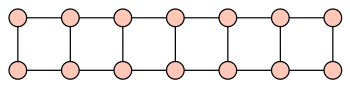
\includegraphics[scale=0.4]{p27.png}\\
$P_{2\times 7}$
\end{center}
Find the number of edge-colorings of $P_{2\times n}$ with $3$ colors. ($P_{2\times n}$ is called \texttt{graphs.Grid2dGraph(2,n)} in Sage).
\end{myex}

\begin{myex}(0pt)
Which topics/theorems/methods from these lectures/exercises did you find most useful/useless/interesting/boring/easy/hard/... \ ?
\end{myex}

\begin{center}
	\line(1,0){330}
\end{center}
Deadline: Friday exam week, 15/04/2016, 23:59.
\end{document}




